\begin{figure*}[tbhp]
  \centering
  % 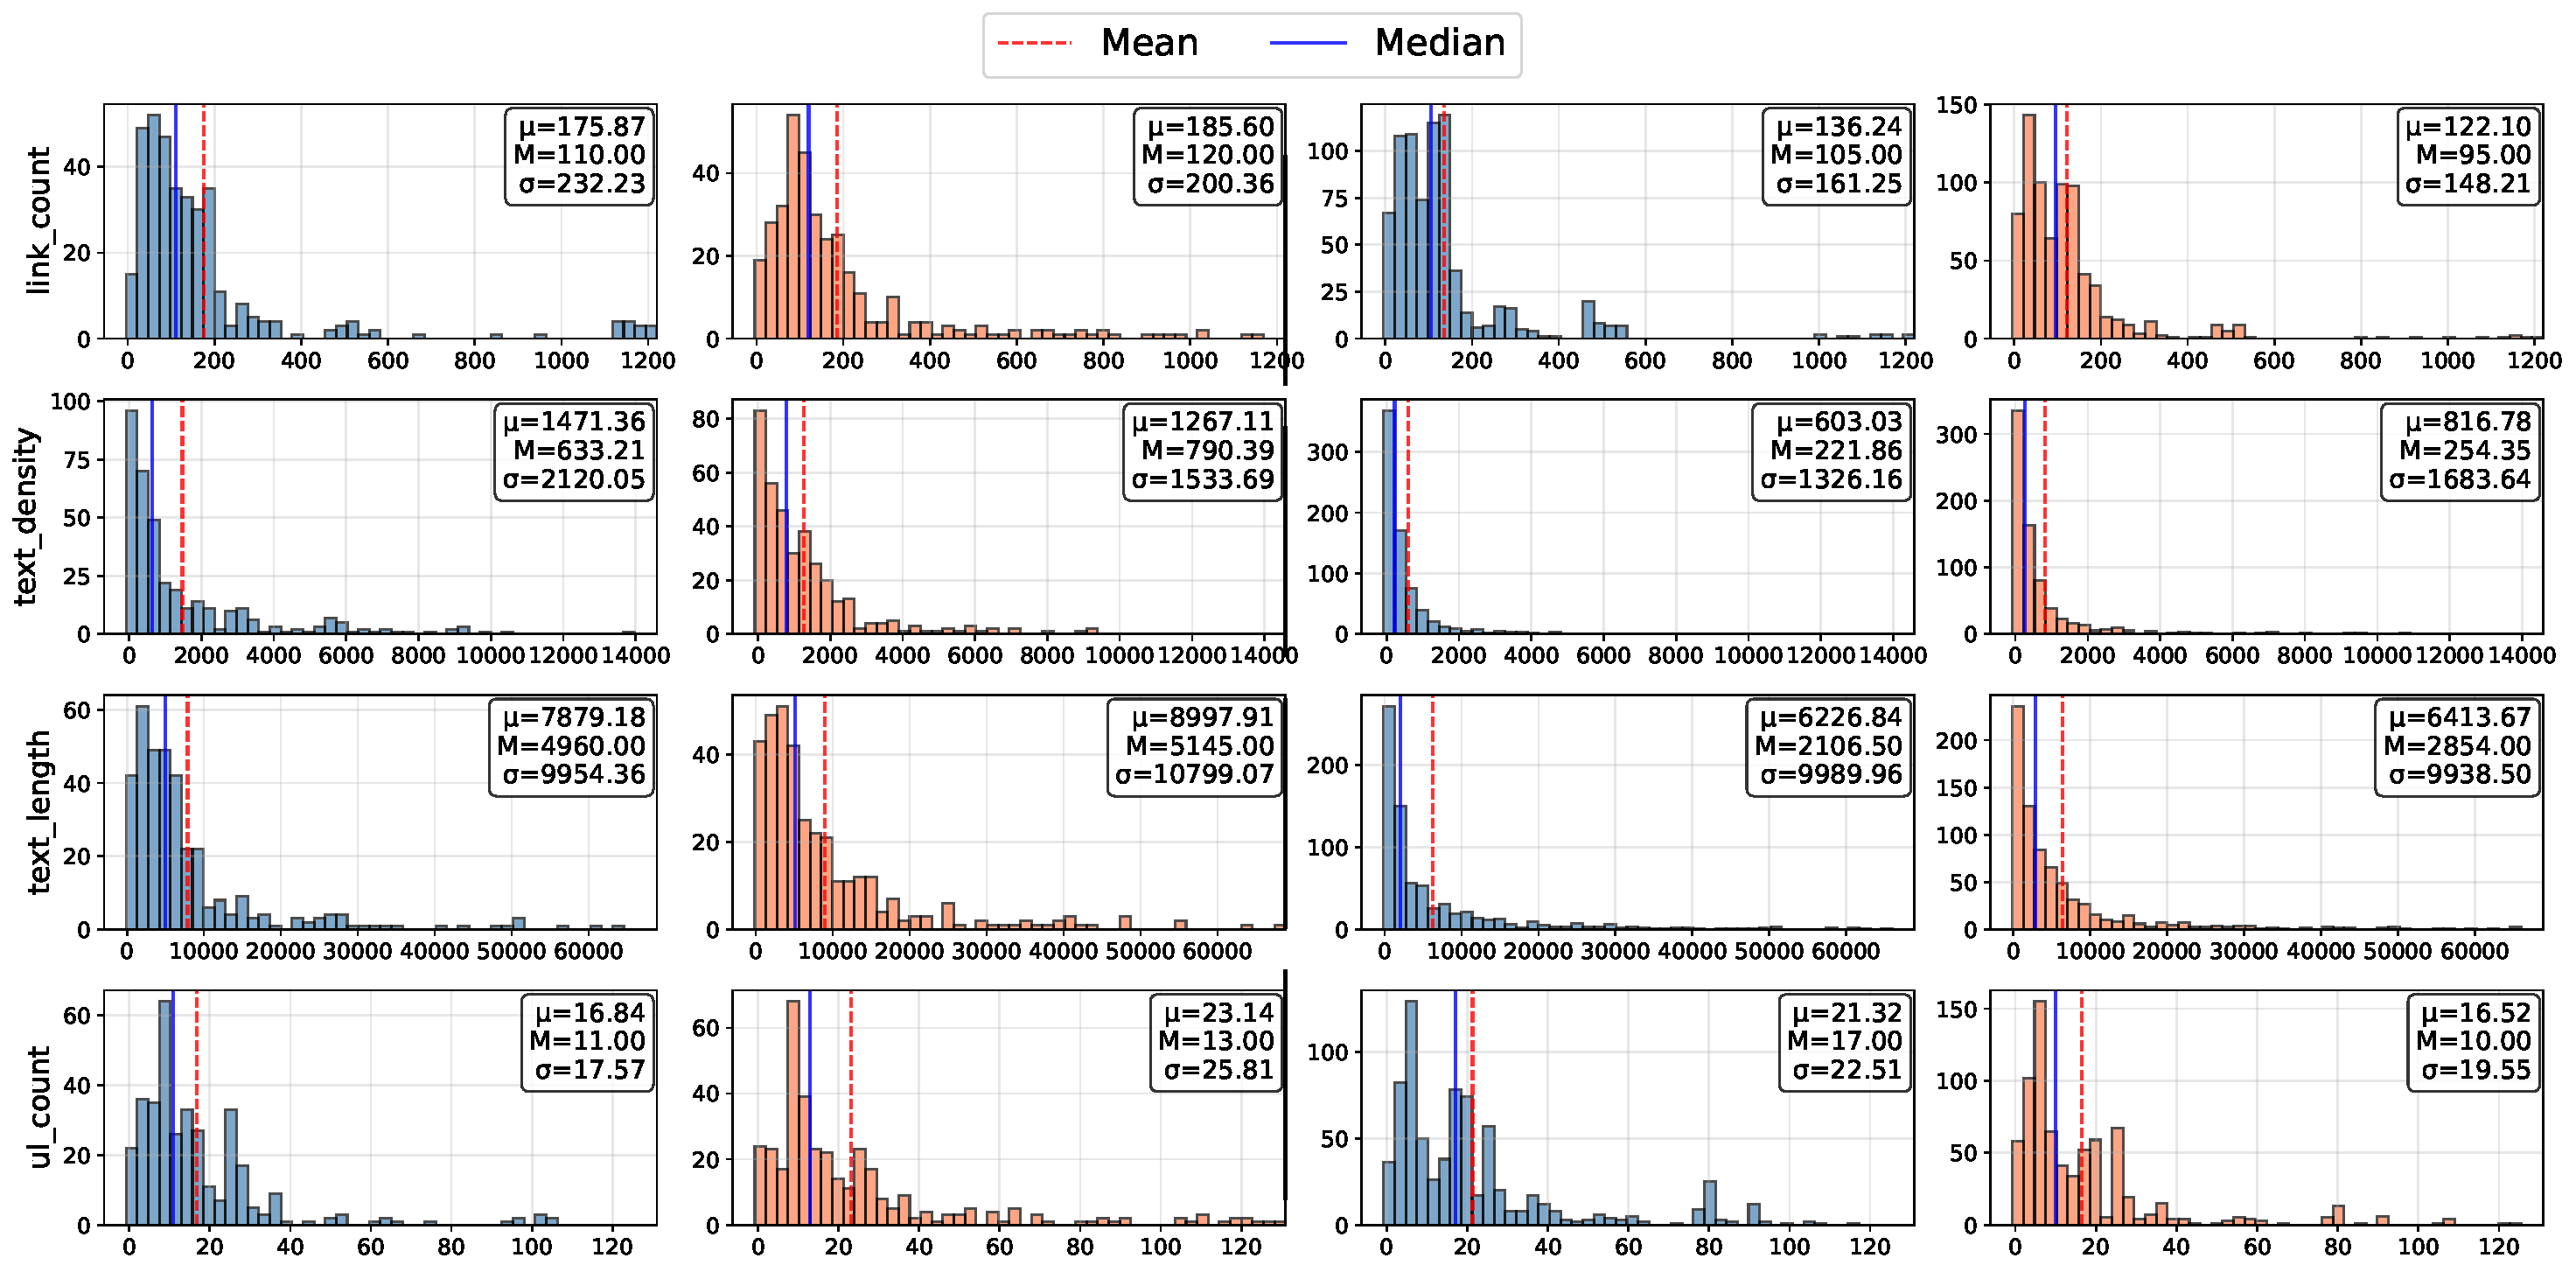
\includegraphics[width=0.85\textwidth]{figs/comparison_histograms_combined_openai.pdf}
  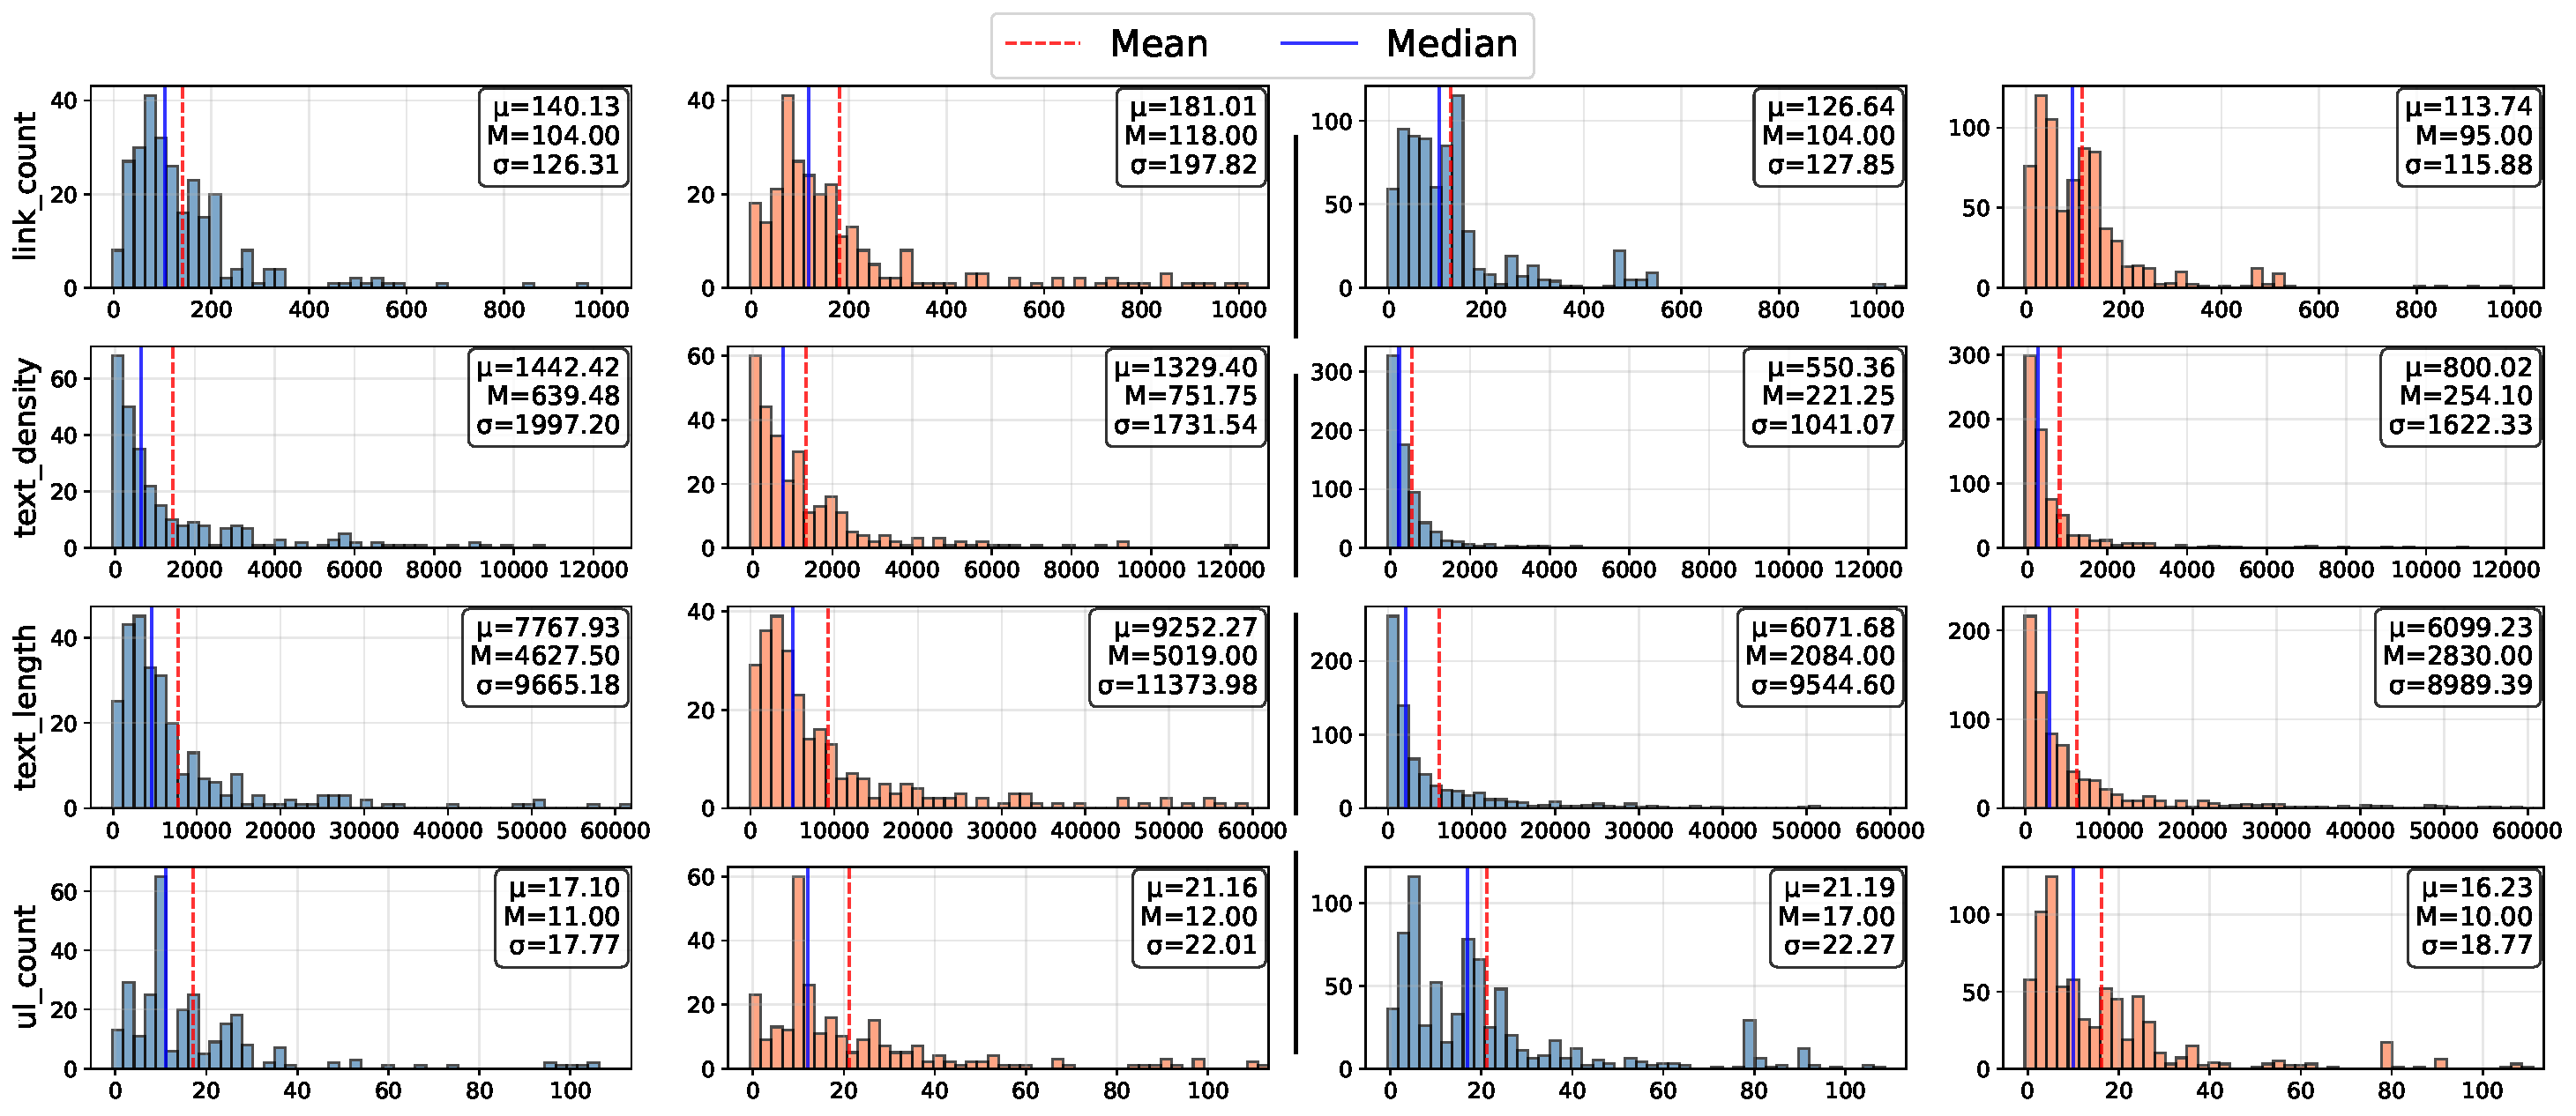
\includegraphics[width=0.90\textwidth]{figs/comparison_histograms_four_columns_openai.pdf}
  \caption{Distribution comparison of web structure features between Citations (left) and Sources (right) for U.S. parties (left two columns) and Japanese parties (right two columns), showing significant differences between cited and non-cited sources}
  \label{fig:comparison_histograms}
\end{figure*}

\section{Analysis of Web Content Structure}
\label{sec:web_analysis}
This section analyzes structural differences between web pages cited by GSEs in their answers and web pages GSEs visited but did not cite, and validates whether these differences align with insights from GEO~\cite{geo-apmr+24} that exposure of web pages as citations depends on the visibility and structure of page text.

\textbf{Experiment Setup: }
% \subsection{Experiment Setup}
\label{subsec:web_experiment_setup}
We limit the target model to GPT-5 because OpenAI's API provides access to both the search result set $S$ and the citation set $C$~\cite{openai-api-reference}, enabling systematic analysis of selection patterns.
Using the results obtained from the experiments in Section~\ref{sec:experiment}, we collect the list of all URLs $ S $ that the GSE visited during web search execution from the search query sequence $ Q^{\prime} = \{q_1, \ldots, q_n\} $ generated by the GSE and extract the citation source sequence $ C $ embedded in response $ r $ (where each $ c_i \in S $).
We conduct the analysis as a two-group comparison between candidates ($ S $) and citations ($ C $), ensuring sufficient sample sizes for closed-ended questions about U.S. political parties (in English) and Japanese political parties (in Japanese) (e.g., U.S. parties $ N = 370 $, Japanese parties $ N = 753 $).

We use four web structure labels as evaluation metrics.
\texttt{link\_count} represents the total number of \texttt{<a>} tags within a page (including external and internal links), whereas \texttt{text\_density} indicates text density per heading hierarchy ($ \text{total\_chars}/\text{number\_of\_}\texttt{<h2>}\text{-to-}\texttt{<h6>}\text{\_tags} $).
\texttt{text\_length} measures the total text volume of the entire page, and \texttt{ul\_count} counts the occurrences of \texttt{<ul>} tags (number of unordered list elements).

To address sample size imbalance, we perform random sampling from the larger group to match the size of the smaller group, ensuring statistical validity.
We evaluate the significance of differences using two types of non-parametric tests:
(i) Mann--Whitney U (MW) test for median differences, and (ii) Kolmogorov--Smirnov (KS) test.
% We set the significance level at $ \alpha = 0.05 $.

\textbf{Results: }
% \subsection{Results}
\label{subsec:web_results}
Figure \ref{fig:comparison_histograms} presents distribution comparisons between Citations ($ C $) and Sources ($ S $) for four metrics in U.S. parties (in English) and Japanese parties (in Japanese).
Table \ref{tab:significance_tests} summarizes the statistical test results for all metrics across both settings.
Key findings align with the GEO study's claims as follows.

Visually inspecting the central tendencies (median and mean) in Figure~\ref{fig:comparison_histograms} further highlights this pattern: while the U.S. results are consistent with GEO's insights, the Japanese results often move in the opposite direction (e.g., shorter \texttt{text\_length} for citations).
For \texttt{link\_count}, cited pages tend to have more links.
Japanese shows significance in both tests, whereas U.S. shows distributional significance.
Numerous links function as gateways to source and related information, supporting evidence presentation by GSEs.
For \texttt{ul\_count}, cited pages exhibit more \texttt{<ul>} tags.
Japanese shows robust significance across tests, whereas U.S. shows median-level effects but limited distributional differences.
\texttt{<ul>} tags reorganize text into point lists, enhancing information readability and extractability, consistent with the GEO perspective.
For \texttt{text\_density}, cited pages have higher text density per heading hierarchy.
U.S. shows significance in distributional tests, whereas Japanese ranges from marginal to significant across tests.
Pages with dense text under appropriately hierarchical headings are more likely to be selected.
For \texttt{text\_length}, Japanese results show that cited pages tend to be shorter,
whereas U.S. shows limited effects.
% Density and structuring through links/\texttt{<ul>} tags contribute to selection more than total volume itself.

Overall, English findings are consistent with GEO, whereas Japanese often shows the opposite trend.
%Structural cues (e.g., \texttt{<ul>} tags, higher \texttt{text\_density}, and more links) increase exposure as citations more than sheer text volume.
These trends could result from several factors, such as differences in bias between languages, linguistic properties, and cultural differences in the structure of persuasive web content.
These findings suggest the necessity of further examination of GEO methods when comparing effectiveness across multiple languages.
% In conclusion, our analysis shows that GEO insights are consistent with our findings and that using these tags increases the exposure of web pages as citations in answers generated by GSEs.



\begin{table}[t]
  \centering
  \caption{Statistical test results for distribution differences}
  \label{tab:significance_tests}
  \begin{tabular}{l cc cc}
    \hline
    & \multicolumn{2}{c}{U.S. parties} & \multicolumn{2}{c}{Japanese parties} \\
    \cline{2-5}
    Metric & MW-$ p $ & KS-$ p $ & MW-$ p $ & KS-$ p $ \\
    \hline
    \texttt{link\_count}   & \textcolor{blue}{0.017*}     & \textcolor{blue}{0.037*}    & \textcolor{blue}{0.042*}    & \textcolor{blue}{0.006**}   \\
    \texttt{text\_density} & 0.257     & \textcolor{blue}{0.015*}    & 0.052     & \textcolor{blue}{0.016*}    \\
    \texttt{text\_length}  & 0.134     & 0.050     & \textcolor{blue}{0.036*}    & \textcolor{blue}{0.008**}   \\
    \texttt{ul\_count}     & \textcolor{blue}{0.039*}     & 0.165     & \textcolor{blue}{< 0.001***}   & \textcolor{blue}{< 0.001***}  \\
    \hline
    \multicolumn{5}{l}{\footnotesize *$ p < 0.05 $, **$ p < 0.01 $, ***$ p < 0.001 $} \\
  \end{tabular}
\end{table}
